\documentclass[../../../main]{subfiles}
\begin{document}

\section{原理}

\subsection{トンネル磁気抵抗効果の概要}
トンネル磁気抵抗(TMR, Tunnnel Magnetoresistance)効果とは、
絶縁体を強磁性体\footnote{
	強磁性体には原子の磁気モーメントが平行に配列することで強い磁化を形成するフェロ磁性(ferromagnetic)と反平行に並べて自発磁化を形成するフェリ磁性(ferrimagnetic)という2つがある。
	フェロ磁性は狭義の強磁性とも呼ばれ、以後は強磁性はこの狭義の強磁性という意味で用いる。
}で挟んだような構造であるMTJ(Magnetic Tunnel Junction)において、
磁化の向きによって電気抵抗が変化する現象である。
磁化の向きが反平行の場合(図\ref{subfig:tmr-ap})、平行の場合(図\ref{subfig:tmr-p})に比べて抵抗が大きくなる。
磁化の向きは外部磁場をかけることで変化させることができ、
前者の場合の抵抗を$R_{AP}$、後者を$R_P$とすれば
\begin{equation}\label{eq:tmr-ratio}
	\text{TMR} = \frac{R_{AP} - R_P}{R_P} \times 100
\end{equation}
で定義される値をTMR比\footnote{
	TMRだけでなくGMR(Giant Magnetoresistance)などと比較する場合には単に、MR比とも呼ばれる。
}呼び、トンネル磁気抵抗効果の大きさを表す指標である。

磁場によって抵抗を変化させる代表的なものとしてGMR(Giant Magnetoresistance)効果に比べると、
\SI{4.2}{K}の低温で(001)Fe($\SI{30}{\AA}$)と(001\footnote{
	(001)はミラー指数である。結晶が立方晶であれば(001)はxy面に平行にFeとCrが積層されていることを意味する。
})Cr($\SI{9}{\AA}$\footnote{
	Crが薄いほどMR比は大きくなる傾向にある。
})の超格子に対して\SI{20}{kG}から\SI{40}{kG}程度でMR比が\SI{50}{\%}であった\cite{gmr}のに対し、
室温で\ce{Al2O3}/Fe/\ce{Al2O3}のMTJに対して\SI{25}{G}から\SI{50}{G}程度で(T)MR比が\SI{20}{\%}程度である\cite{tmr}。
つまり、より小さい磁場で大きなMR比を得ることができるという利点があった。
いまではさらに研究が進み、室温で200\%を超えるTMR比を得る\cite{tmr-aist}\cite{tmr-mgo}ことができる。
\begin{figure}
    \centering
    \begin{subfigure}{0.48\linewidth}
        \centering
        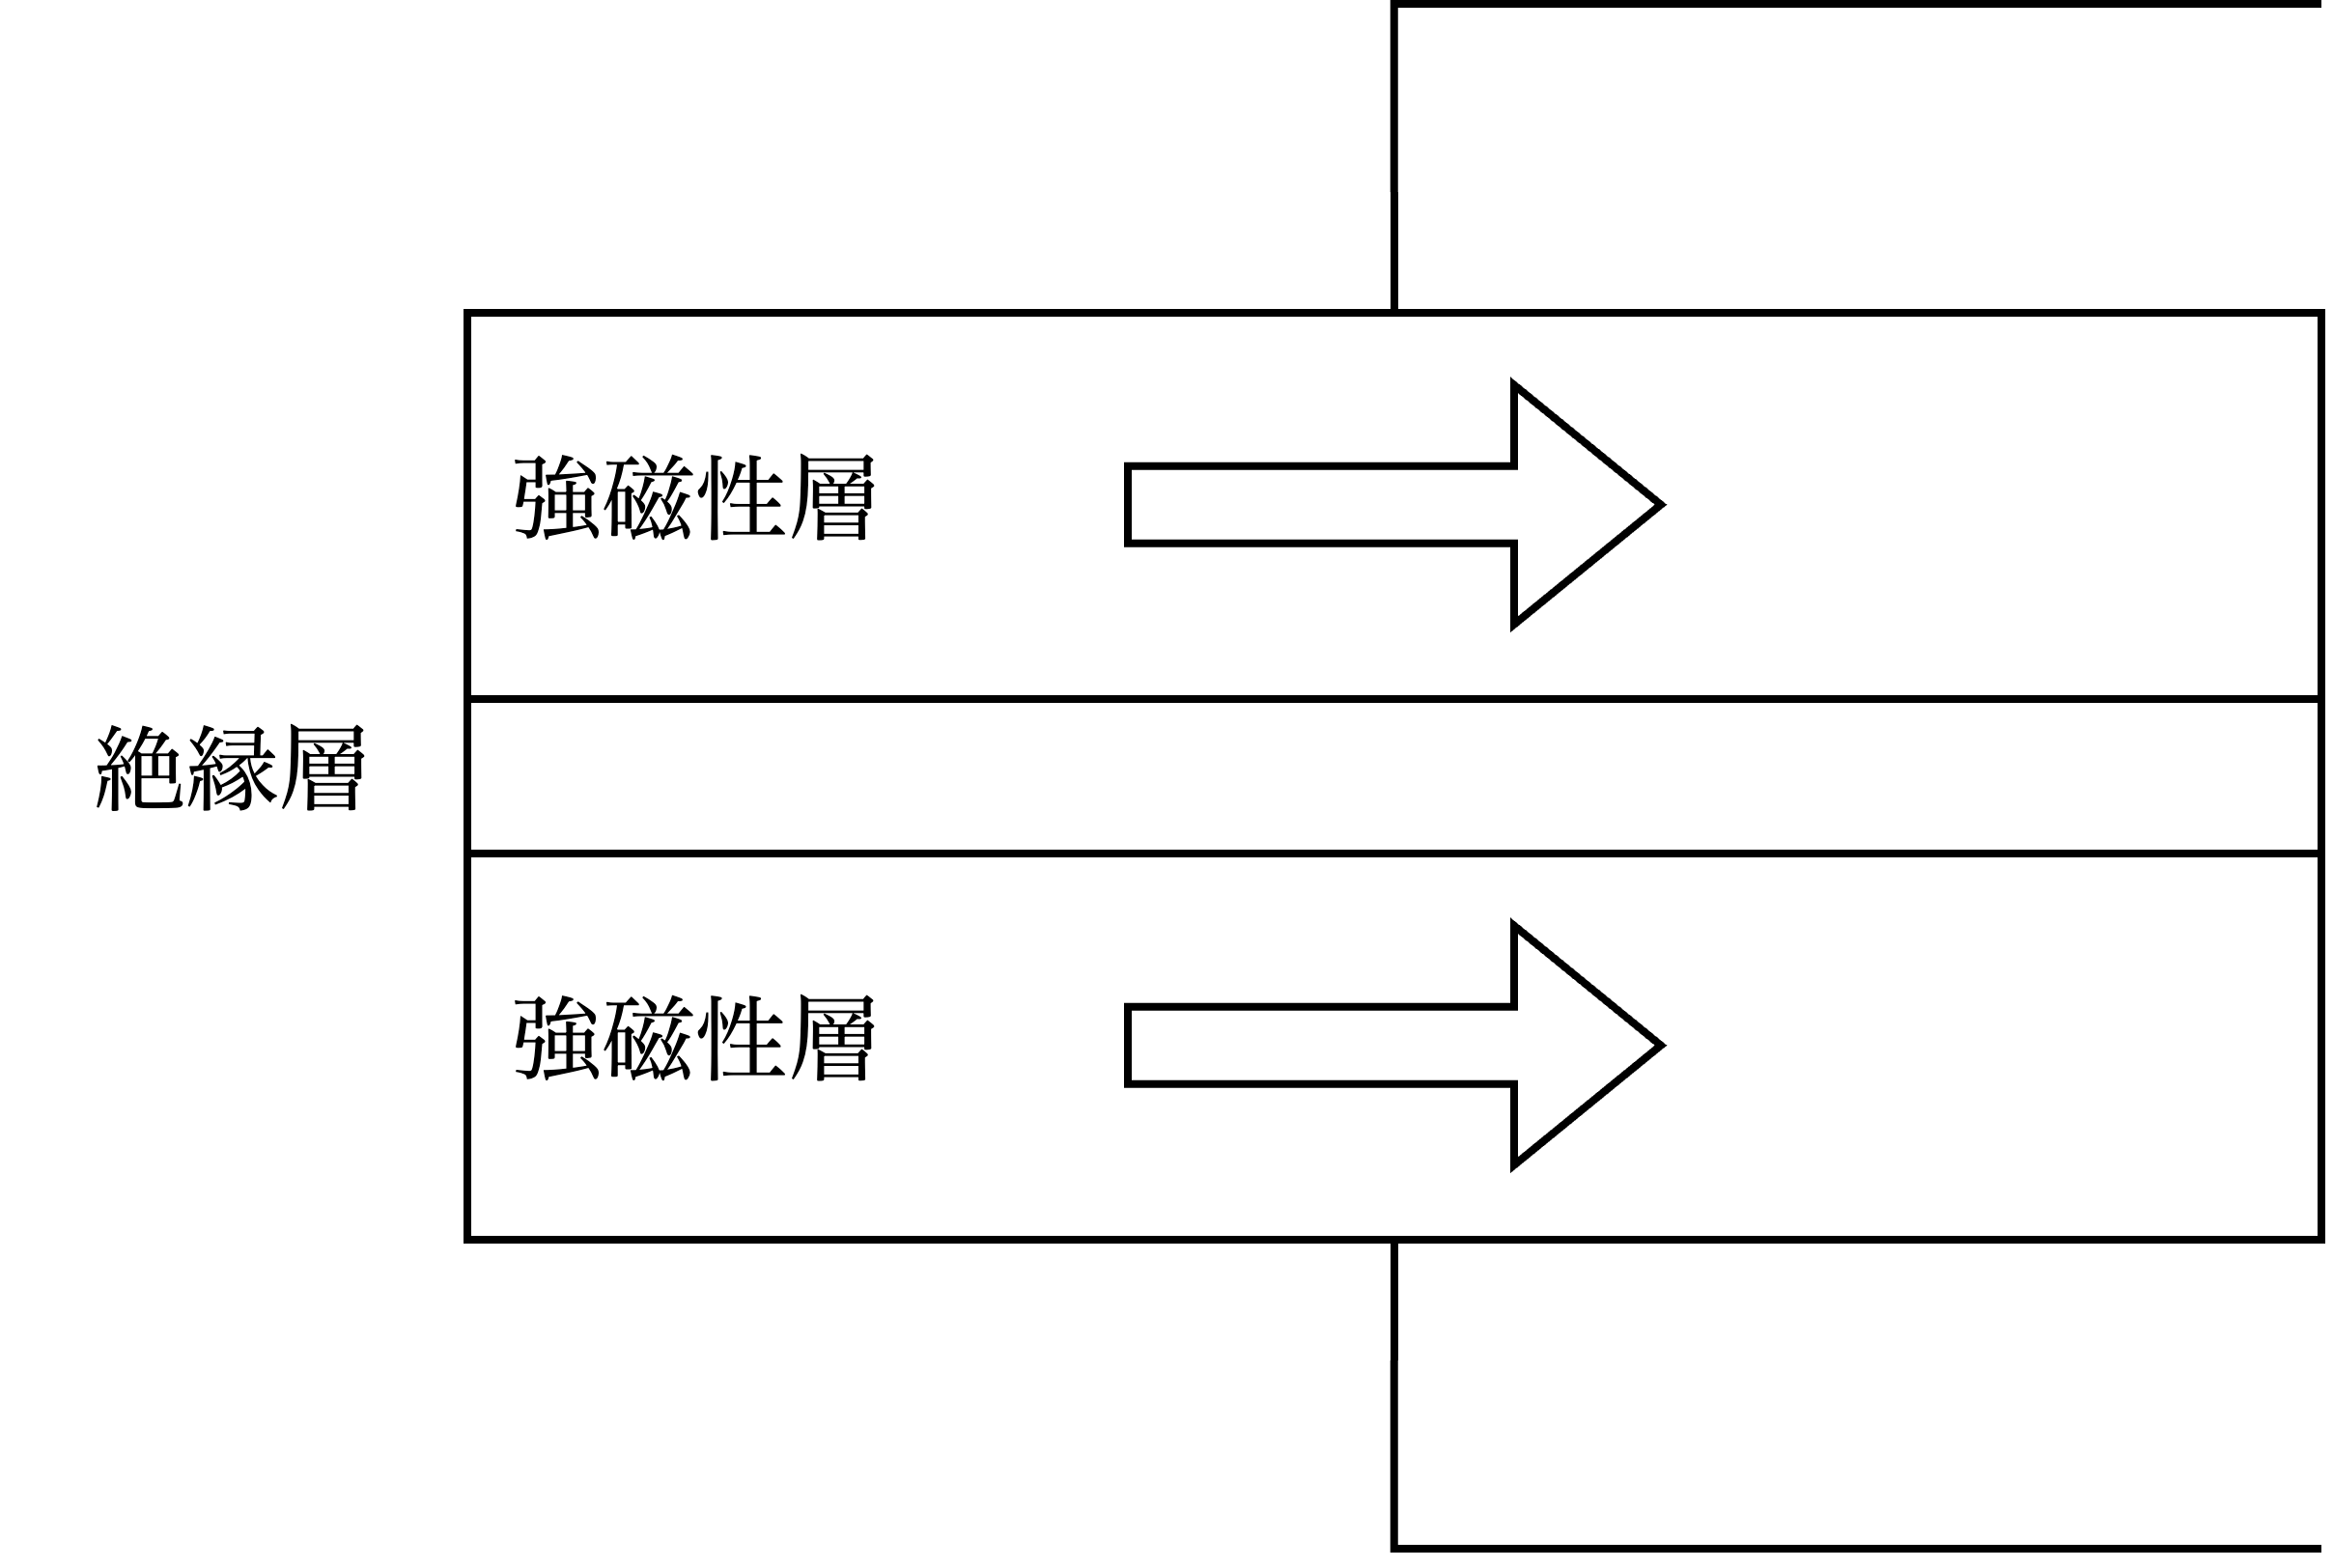
\includegraphics[width=0.8\linewidth]{src/figures/pri-tmr/tmr-p.png}
        \subcaption{磁化が平行の場合}\label{subfig:tmr-p}
    \end{subfigure}
    \begin{subfigure}{0.48\linewidth}
        \centering
        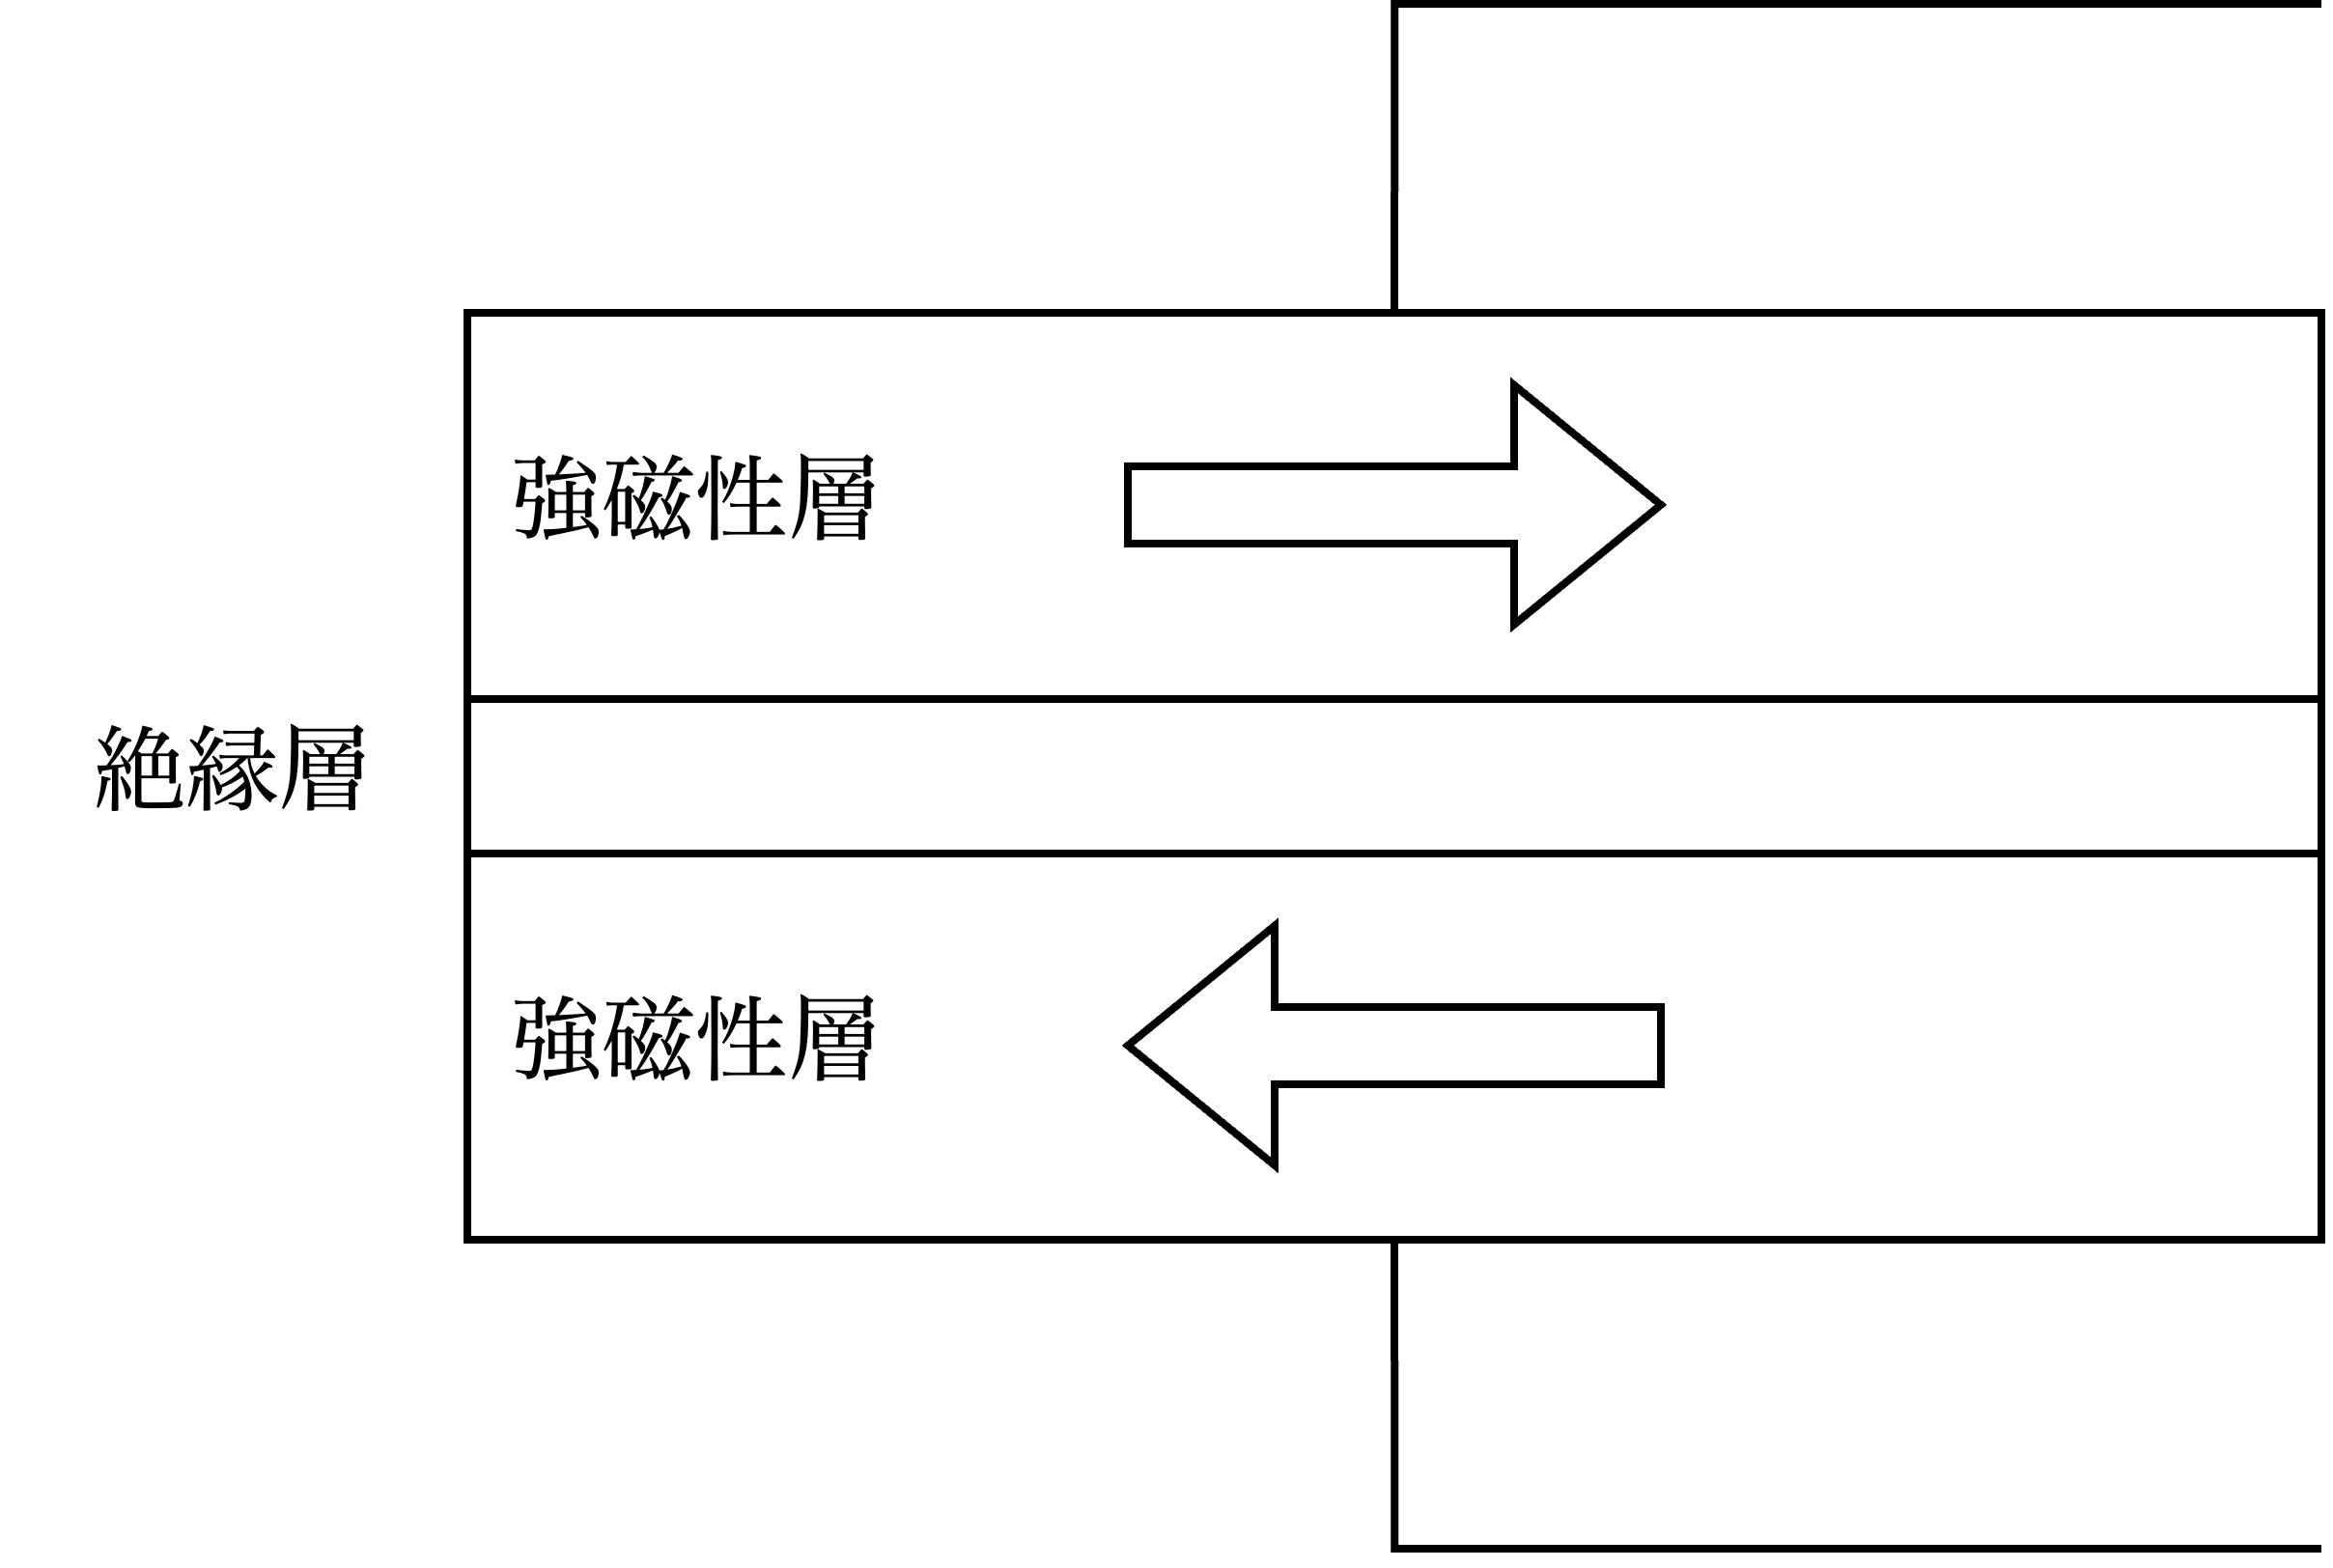
\includegraphics[width=0.8\linewidth]{src/figures/pri-tmr/tmr-ap.png}
        \subcaption{磁化が反平行の場合}\label{subfig:tmr-ap}
    \end{subfigure}
    \caption{MTJ(Magnetic Tunnel Junction)におけるTMR(Tunnel Magnetoresistance)効果}\label{fig:pri-tmr}
\end{figure}


\subsection{トンネル磁気抵抗効果の機構}
TMR効果の機構の説明にはJulliereが提唱したモデル\cite{julliere-model}がしばしば用いられる。
金属中で電子が自由粒子であり3次元空間中を移動するとすると、DOSは$\sqrt{\epsilon}$に比例し分布はフェルミ分布関数に従う。
MTJの強磁性層が平行のとき(P state)と半平行のとき(AP state)のバンド図を図\ref{fig:tmr-dos}に示す。\footnote{
	この図では、up spinがmajority spin、down spinがminority spinとして図示してある。
}
電子は左側の強磁性層からトンネル効果で絶縁層を通過し、右側の強磁性層に入るとする。
主にフェルミ面付近の電子が電気伝導に寄与するためその部分に注目すると、
Pstateでは$D^{P}_{L\downarrow}$と$D^{P}_{R\downarrow}$が大きいため上向きスピンのトンネル電流が大きく、
逆にAPStateでは、$D^{AP}_{L\downarrow}$は大きいが、$D^{AP}_{L\downarrow}$は小さいため上向きスピンのトンネル電流は小さく、
$D^{AP}_{L\uparrow}$は小さいため、$D^{AP}_{R\uparrow}$は大きいにもかかわらず下向きスピンのトンネル電流も小さい。
このとき、トンネルコンダクタンス$G_P$、$G_{AP}$は
\begin{equation}\label{eq:tmr-g-p}
	G_P \propto D^{P}_{L\downarrow}(\epsilon_f)D^{P}_{R\downarrow}(\epsilon_f) + D^{P}_{L\uparrow}(\epsilon_f)D^{P}_{R\uparrow}(\epsilon_f)
\end{equation}
\begin{equation}\label{eq:tmr-g-ap}
	G_{AP} \propto D^{AP}_{L\downarrow}(\epsilon_f)D^{AP}_{R\downarrow}(\epsilon_f) + D^{AP}_{L\uparrow}(\epsilon_f)D^{AP}_{R\uparrow}(\epsilon_f)
\end{equation}
と表される。
これらの比例係数は同じであるとして、TMR比は
\begin{align}\label{eq:spin-polarization}
	\textrm{TMR} & = \frac{1/G_{AP} - 1/G_P}{1/G_P} \nonumber                                         \\
	             & = \dfrac{(D_{\uparrow} - D_{\downarrow})^2}{2D_{\uparrow}D_{\downarrow}} \nonumber \\
	             & = \dfrac{2P^2}{1 - P^2}
\end{align}
とかける。
ここで、$D_{\uparrow}=D^{P}_{L\uparrow}=D^{AP}_{L\uparrow}=D^{P}_{R\uparrow}=D^{AP}_{R\downarrow}$などであり、
$P=\dfrac{D_{\uparrow}-D_{\downarrow}}{D_{\uparrow}+D_{\downarrow}}$であり、この$P$をスピン分極率という。\footnote{
このモデルではMajority Spinを上向きスピンとしているから、$P>0$にとればTMRからスピン分極率が求まる。
一般には、$D_{\uparrow}$を$D_{major}$、$D_{\downarrow}$を$D_{minor}$として、$P=\dfrac{D_{major}-D_{minor}}{D_{major}+D_{minor}}$とする。
}

\begin{figure}
    \centering
    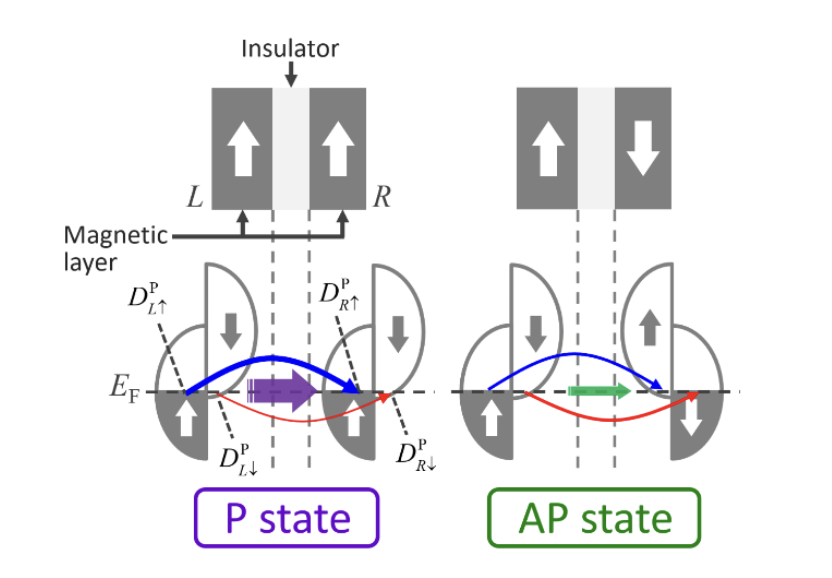
\includegraphics[width=0.6\linewidth]{src/figures/tmr-dos/tmr-dos.png}
    \caption{トンネル磁気抵抗効果の機構(\cite{kaiju}より)}\label{fig:tmr-dos}
\end{figure}


\subsection{ヒステリシス環線}\label{subsec:hysteresis-loop}
強磁性体は磁場によって強く磁化し、透磁率は大きい。
この透磁率は磁場の強さによって変化し、非線形特性を示す。
このため一般に強磁性体の磁化$I$は磁場$H$によって複雑に変化しその様子を磁化曲線という。
強磁性体は$H=0$、$I=0$という消磁状態から始まり$H$を増加させると、$I$も増加していく。
ある点Aで磁化は可逆的ではなくなり、この点Aから$H$を減少させると再び点Oに戻ることができるが、この点を超えると不可逆的となる。
さらに増加させていくと、飽和状態に達し$H$に対して$I$は一定値に近づく。
消磁状態から$H$を増加させ飽和状態に達したのち、$H$を小さくしても元の曲線は辿らず、
$H=0$の状態でも磁化が残る。
これを残留磁化という。
さらに$H$を小さくしていくと、マイナスの飽和状態へと達する。
その後、$H$を増加させると$H=0$でマイナスの残留磁化がのこりプラスの飽和状態へと至る。
この一週の曲線をヒステリシス環線(Hysteresis Loop)という。\cite{ferromagnetic}
図\ref{fig:hysteresis-loop}にヒステリシス環線の例を示す\footnote{
	この図では、点Aが磁化が可逆な$H$の限界、点Bが飽和状態、点Cの$I$が残留磁化、点Dの$H$の値を保持力(Coercive force)、点Fがマイナスの残留磁化を表している。
}。
したがって、MTJのTMR比を測定するためにはMTJに磁場をかけて強磁性体の磁化を変化させる必要があるがその磁化はどのように磁場を変化させたかに依る。
\begin{figure}
    \centering
    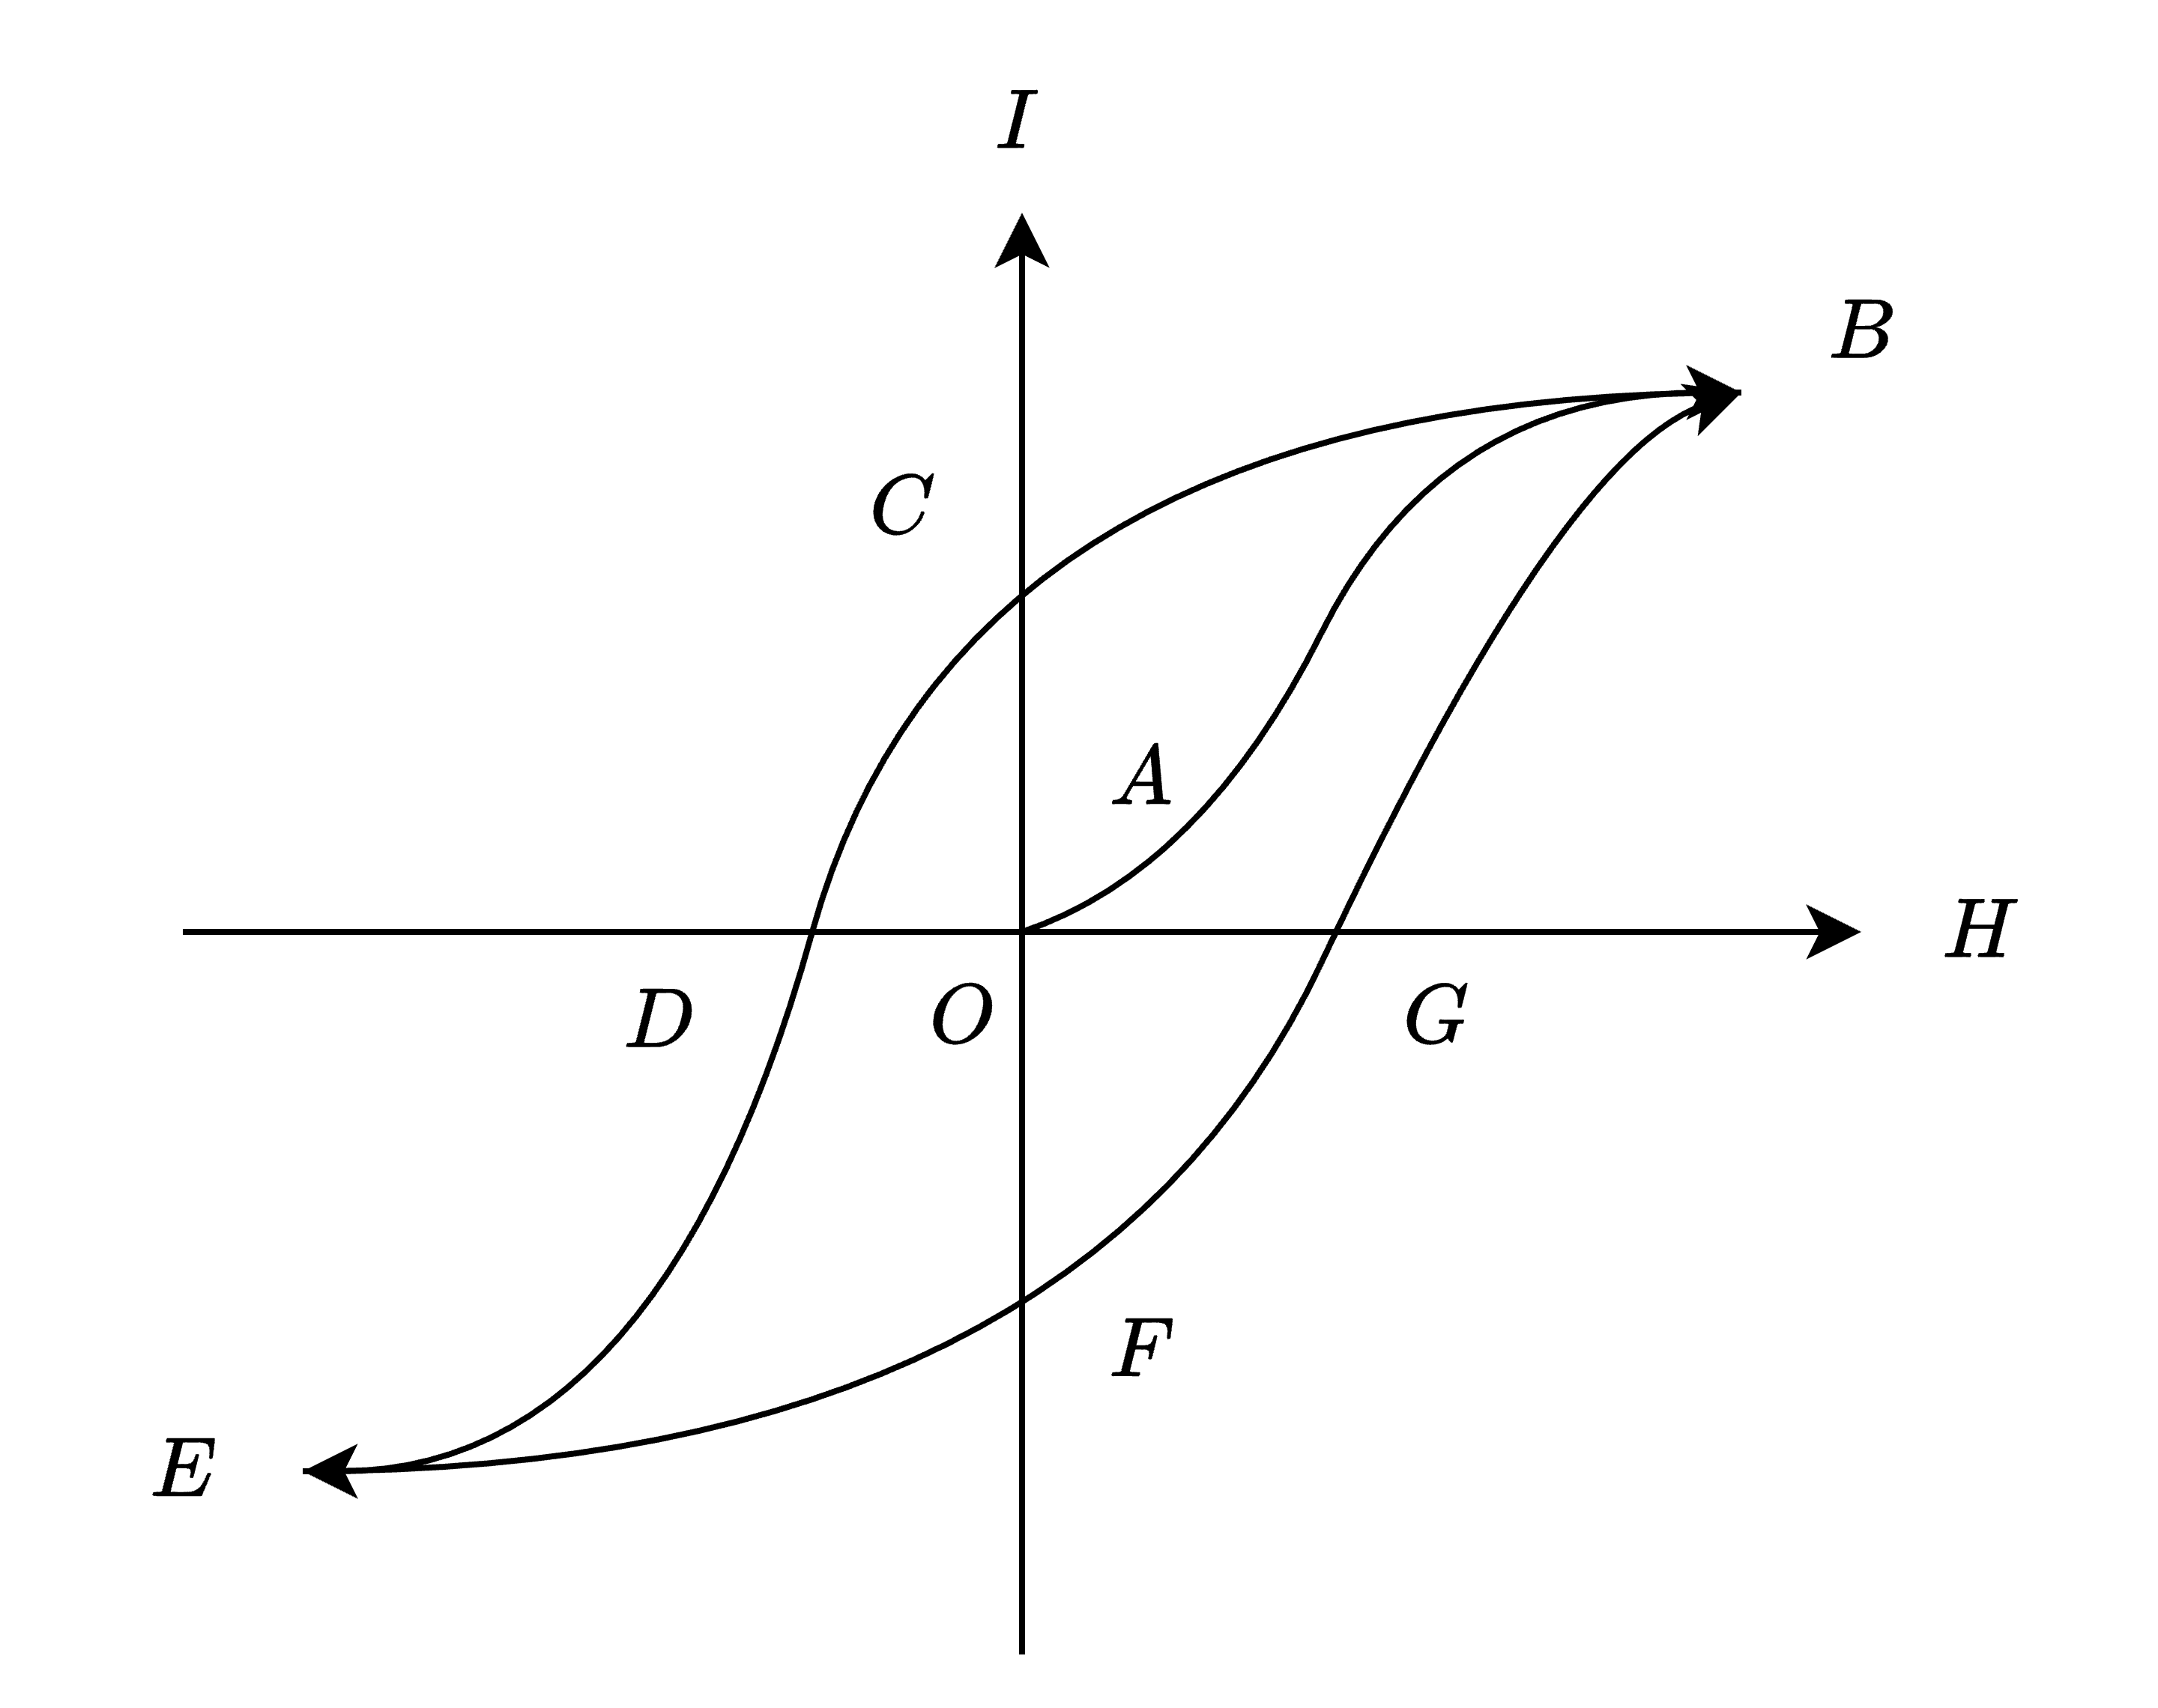
\includegraphics[width=0.5\linewidth]{src/figures/hysteresis-loop/hysteresis-loop.png}
    \caption{Hysteresis Loop}\label{fig:hysteresis-loop}
\end{figure}








\end{document}
